\documentclass{ledger}


\overfullrule=10pt

\title{Descriptive Title Written in Twenty-four Point Times New Roman}
\author{First A.~Author\thanks{F.~A.~Author (first@stanford.edu) is Professor of Computer Science at Stanford University, USA}\and Second B.~Author\thanks{S.~B.~Author\textellipsis author affiliations should be written in 8 pt.~Times New Roman font and 9pt.~line spacing}\and 13 pt.~Times New Roman}

\begin{document}

\maketitle

\begin{abstract}
The abstract should be written in 10 pt.~ Times New Roman font, 13 pt.~line spacing, and 1.2 cm indenting on either side.  Give a concise summary of the paper in a single paragraph of approximately 150 words (200 words max).  The abstract should communicate both what the paper is about and the important results obtained.  The abstract should contain neither references nor non-plain text elements such as equations or compute code.

\begin{keywords}
\item First key word
\item Second key word
\item Same style as abstract
\item Not more than two lines of keywords
\end{keywords}
\end{abstract}

\section{Introduction (13 pt.\ Times New Roman Bold)}

Body text should be written in 11 pt.\ Times New Roman font with 13pt.\ line spacing.  The first paragraph and the headings and sub-headings should not be indented, but subsequent paragraphs should be indented 0.6cm.

The first body section must be labeled ``Introduction''  Using plain language, explain why your work is important, describe how it fits within the existing body of cryptocurrency knowledge, and then state in what way your work represents a new contribution.  If your paper does not follow a conventional structure (see below), then the Introduction should end by describing what the following sections of the paper are about.  The Introduction should contain approximately 500 to 750 words (1000 words max) and should not use sub headings.

\section{Body Section Headings are 13pt.\ Times New Roman Bold}

Any number of body sections may follow the Introduction.  For hypothesis-driven research, we suggest the conventional structure of Methods, Results, Discussion.  For technology-advancement papers, provide concise descriptive titles for each body section.  The body sections should logically flow together such that the paper tells a cohesive and compelling story of the research that was undertaken and the results that were obtained.


\subsection{Subheadings are inline and written in italic and followed by an em dash}

Sub headings should be used sparingly but are appropriate where a sequence of more or less unrelated material (particularly in a long Methods section) may flow better.

\subsection{Page margins}

\emph{Ledger} uses right and left page margins of 3.1 cm, and top and bottom margins of 2.4 cm and 1.0 cm, respectively.  Headers and footers are, respectively, 1.5 cm and 1.0 cm from the edge.  The bottom footer overlaps with the bottom page margin, and has the effect of pushing the effective bottom margin up on each page after the first, thereby placing the author affiliations in a more appropriate location closer to the bottom of the first page.

\subsection{Tables}

\cref{tbl:1} is an example of a properly formatted table.  It also describes the styles used in this document.

\begin{table}[ht]
\caption{Fonts and Paragraph Styles.}\label{tbl:1}
\begin{tabularx}{\textwidth}{ l  c  c  C  C  C  c  c  c  c }
\hline
\tableheading{Style name} & \tableheading{Font} & \tableheading{Size \\ \centering (pt.)} & \multicolumn{3}{c}{\tableheading{Paragraph spacing \\ \centering (pt.)}} & \tableheading{Bold} & \tableheading{Italic} & \tableheading{All \\ \centering caps} & \tableheading{Center- \\ \centering ed} \\ \cline{4-6}
 & & & \fontsize{8pt}{8pt}\selectfont Line & \fontsize{8pt}{8pt}\selectfont Above & \fontsize{8pt}{8pt}\selectfont Below & & & & \\\hline
Article title & Times & 24 & 28 & 0 & 0 & $\square$ & $\square$ & $\square$ & $\blacksquare$ \\
Authors names & Times & 13 & 13 & 14 & 20 & $\square$ & $\square$ & $\square$ & $\blacksquare$ \\
Author affiliations & Times & 8 & 9 & 0 & 1 & $\square$ & $\square$ & $\square$ & $\blacksquare$ \\
Abstract\footnote{The Abstract section begins with the word ``Abstract'' in bold face and followed by a period.  The abstract text immediately follows (no line break) and has regular font weight.} & Times & 10 & 13 & 0 & 0 & $\square$ & $\square$ & $\square$ & $\square$ \\
\pbox[c][.8cm]{\textwidth}{Article type / ``Key \\ words'' heading} & Times & 10 & 13 & 9 & 6 & $\square$ & $\square$ & $\blacksquare$ & $\blacksquare$ \\
Section headings & Times & 13 & 15 & 15 & 7 & $\blacksquare$ & $\square$ & $\square$ & $\square$ \\
Sub headings\footnote{Subsections are allowed and can be numbered or unnumbered.  In either case, the heading is written in-line with the body text and in italic followed by an em dash.} & Times & 11 & 13 & 0 & 0 & $\square$ & $\blacksquare$ & $\square$ & $\square$ \\
Body text & Times & 11 & 13 & 0 & 0 & $\square$ & $\square$ & $\square$ & $\square$ \\
Figure captions & Times & 10 & 13 & --- & 20 & $\square$ & $\square$ & $\square$ & $\square$\footnote{Figure captions less than one line in length should be centered while multi-line captions should be justified.} \\
Table captions & Times & 10 & 13 & 15 & 6 & $\square$ & $\square$ & $\square$ & $\blacksquare$ \\
Text in tables & Times & 10 & 12 & 1 & 1 & $\square$ & $\square$ & $\square$ & --- \\
Table headings & Times & 10 & 13 & 4 & 4 & $\square$ & $\square$ & $\square$ & $\blacksquare$ \\
Text in figures & Arial & 8 & --- & --- & --- & $\square$ & $\square$ & $\square$ & --- \\
References & Times & 10 & 12 & 0 & 6 & $\square$ & $\square$ & $\square$ & $\square$  \\
Footnotes in tables & Times & 8 & 11 & 0 & 3 & $\square$ & $\square$ & $\square$ & $\square$ \\
Code & Courier New & 10 & 11 & 0 & 0 & $\square$ & $\square$ & $\square$ & $\square$ \\
Display equations & \makebox[0pt]{\pbox[c][.8cm]{\textwidth}{Times or \\ \centering Cambria Math}} & 12 & --- & 9 & 7 & $\square$ & $\square$ & $\square$ & $\blacksquare$ \\ \hline
\end{tabularx}
\end{table}

\subsection{Numbered and bulleted lists}

Authors are encouraged to use lists to improve the readability of information best presented in point form.  The requirements are as follows.
\begin{enumerate}
\item The line marker is indented 0.6 cm.
\item The list item is further indented 0.6 cm (1.2 cm) in total.
\item If the item is longer than a single line, the text on wrapping lines must begin at an indentation of 1.2 cm, and the line spacing must be consistent with the body of the text.
\item If the list is ordinal, the numbers (or letters) must be surrounded by round brackets.
\item For non-ordinal lists, use small round dots as markers.
\end{enumerate}
Nested lists are permissible but should be used sparingly.

\subsection{Figures}

\cref{fig:1} is an example of a figure.  Figures should be of sufficient resolution (300 DPI for photographs and 600 DPI for line art).

\begin{figure}[ht]
\centering
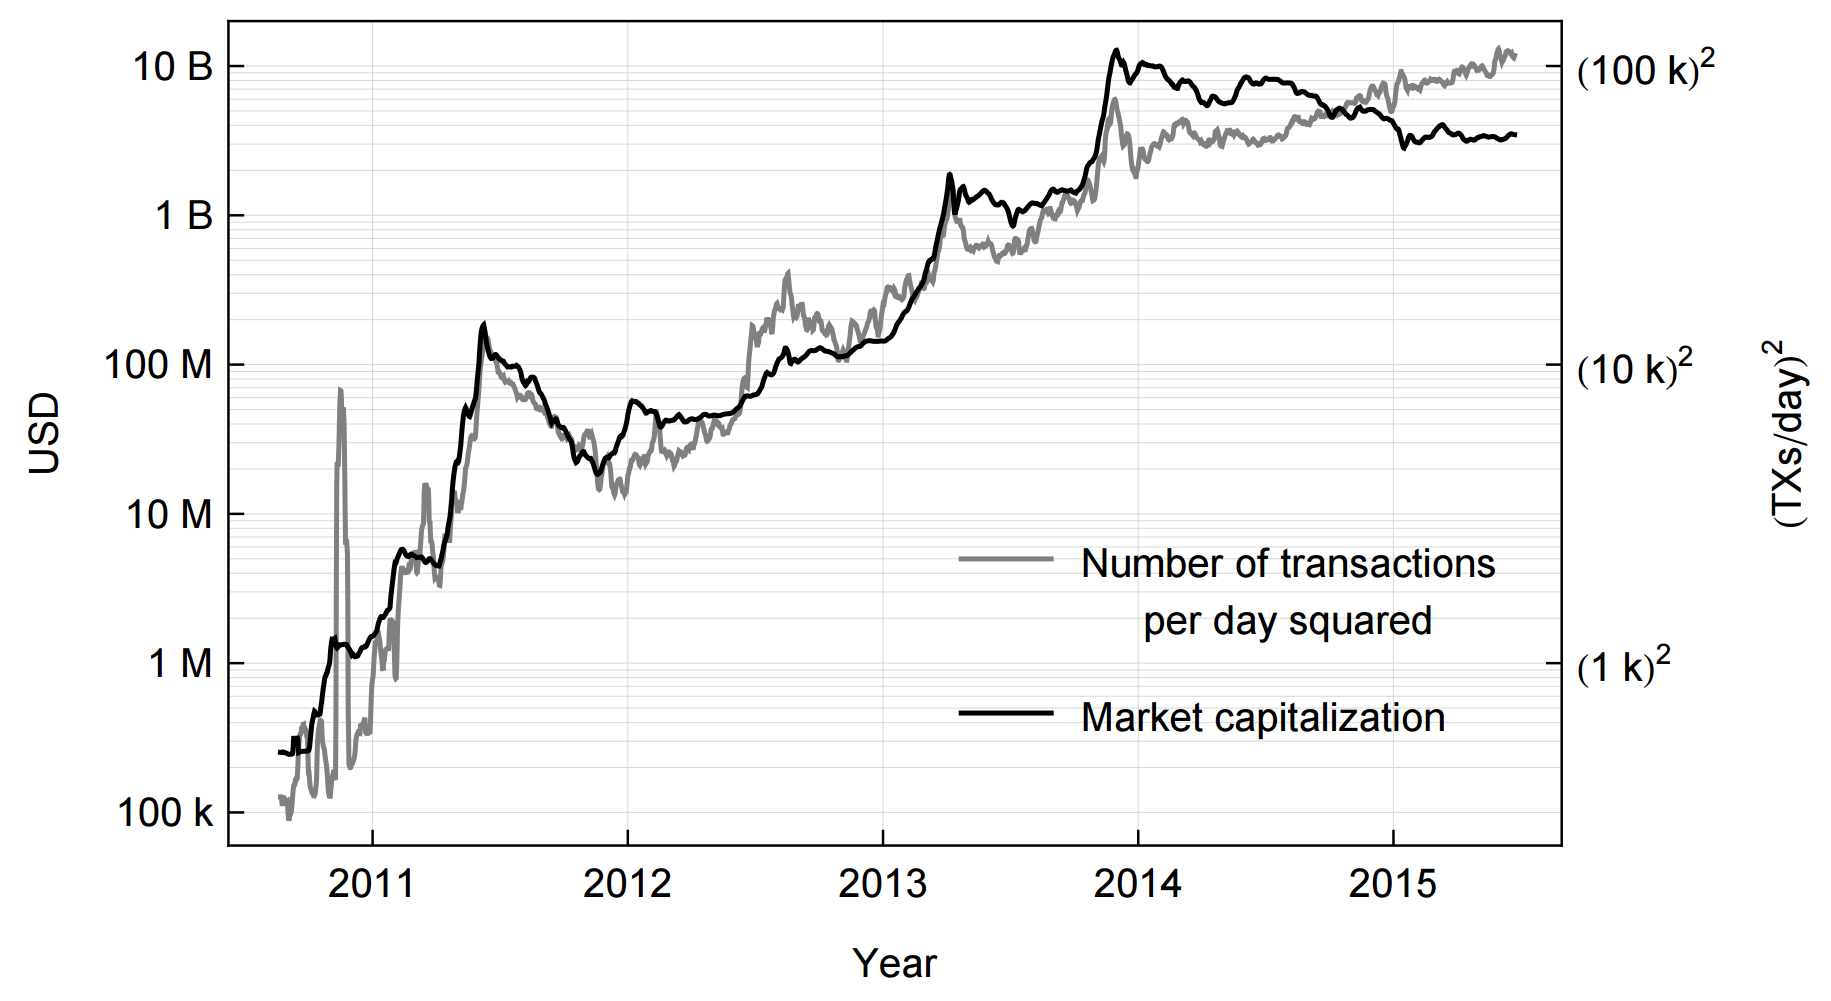
\includegraphics[width=5in]{graph}
\caption{This is an example of an acceptable plot.  The axes are clearly labeled, 8 pt.\ Arial font is used, gridlines are faint ($1/4$ pt.), the plot frame is slightly thicker ($1/2$ pt.\ black) and the plotted data heavier still ($1$ pt.).  In this example, gray scaling is used to differentiate between the two time series.}
\label{fig:1}
\end{figure}

\subsection{Mathematical equations}

Equations should appear inline whenever possible however, equations that are important, referenced in another place in the text, or complex should be centered and displayed separated from teh surrounding text by 9 pts.\ of white space above and 7 pts.\ of white space below:
\begin{equation}
P_{\text{doublespend}}=1-\sum _{k=0}^za\frac{\lambda ^ke^{-\lambda}}{k!}\left[ 1-(q/p)^{z-k}\right] .
\end{equation}
Authors submitting in Microsoft Word must use the built-in equation editor of the MathType plug-in.



% \begin{theorem2}
% This is an important theorem.
% \end{theorem2}


\begin{theorem}
Let $f$ be a function whose derivative exists in every point, then $f$
is a continuous function.
\end{theorem}

\begin{myproof}
Here is my important proof
\end{myproof}

\begin{lemma}
Given two line segments whose lengths are $a$ and $b$ respectively there
is a real number $r$ such that $b=ra$.
\end{lemma}





\subsection{Code}

Code segments can be displayed inline using 10 pt.~Courier New (e.g., \lstinline|#define largerlimit 8000000|), or on display in the same font:
\begin{lstlisting}
if(blocknumber > 115000)
maxblocksize = largerlimit
\end{lstlisting}
For displayed code, the first line should be indented by 1.2cm (twice the standard indent) with additional tabs at multiples of 0.6 cm.

\subsection{Endnotes}

Endnotes are denoted with a superscript Arabic numeral and ordered sequentially.  The final section of the manuscript lists the notes and references (i.e., the endnotes) denoted throughout the paper.  Notes provide proof of facts stated in the article, or additional clarifications on points made in the manuscript.  References list cited material; for example, this is a reference to a journal article,\endnote{Wilmer, C.~E., Rizum P.~R.  ``How to Write and Format an Article for \textit{Ledger}.''  \textit{Ledger} \textbf{1.1} 1--11 (2015) doi:10.1037/rmh0000008} this is a reference to a book,\endnote{Wilmer, C.~E. \textit{Ledger:  The Story of a Journal}.  Pittsburgh:  University of Pittsburgh Press 32--33 (2016).} this is a reference to a forum comment,\endnote{Wilmer, C.~E.~(/u/ThorwawayLedgerAcct).  Comment in ``On the Future of Bitcoin.''  \textit{Reddit} (accessed 11 January 2016) https://www.reddit.com/r/bitcoin/comments/3iao3i/on\_ the\_ future\_ of\_ bitcoin/cupd80} and this is a reference to the Bitcoin white paper.\endnote{Nakamoto, S.~``Bitcoin:  A Peer-to-Peer Electronic Cash System.''  No Publisher (2008) https://bitcoin.org/bitcoin.pdf}

\section{Conclusion}

For papers that do not follow a conventional structure, synthesize and summarize the main results of the paper.  This section is also an appropriate place to clarify the limitations of the work, as well as to describe new research questions that arose.  The conclusion section for papers that follow a conventional structure (i.e., Methods, Results, Discussion) may be very short because the synthesis of the results usually occurs in the Discussion section.  The Conclusion and the Introduction should be the two sections of your paper most accessible to an interdisciplinary readership.

\section{Acknowledgement}

Acknowledge people who helped carry out the research or prepare the manuscript but whose contribution did not warrant authorship.  List funders and other sources of financial support at the end of this section.

\section{Author Contributions}

State the contribution made by each author.  Refer to authors using their initials, for example, ``FAA developed the code to perform the simulation (65\% ) and SBA analyzed the results (35\% ).  They both contributed equally to manuscript preparation.''

\section{Conflict of Interest}

State any potential conflict of interest here, again referring to authors using their initials.  Although assessing whether a conflict of interest exists can be difficult, as a guideline consider whether it would be embarrassing should the potential conflict become publicly known.  This section may be omitted if no conflict of interest exists.

\appendix

\section{Calculations}

Relegate to an appendix material that would distract from the flow of the article, but that is required to rigorously prove claims made or concepts introduced in the paper’s body.

\theendnotes

\end{document}
